\subsection{Erwartungswerte}

Interpretiert man eine Zufallsvariable als ein Experiment mit einem zufälligen Ausgang, so könnte man sich überlegen, welche Methoden sich zur Berechnung des Erwartungswertes anbieten.

\begin{Beispiel}{(Erwartungswert Würfel)}
Wir betrachten wieder das \hyperlink{Bsp:Würfel}{\blue{Würfelbeispiel}}. Naiv würde man berechnen, dass man mit einer Wahrscheinlichkeit von $1/6$ die Zahl Eins würfelt, mit $1/6$ die Zwei und so weiter. Wir berechnen also
\[1 \cdot \frac{1}{6} + 2 \cdot \frac{1}{6} + 3 \cdot \frac{1}{6} + 4 \cdot \frac{1}{6} + 5 \cdot \frac{1}{6} + 6 \cdot \frac{1}{6} = 3.5~.\]
Ist $E = \{1, \dots, 6\}$ unser Ergebnisraum, so berechnen wir
\[\mathbb{E}(X) = \sum_{n \in E} n \mathbb{P}(X = n)~.\]
Vergleichen wir dies mit unserem \hyperlink{Kor:Dichtekorollar}{\blue{Dichtekorollar}}, so könnte man auf die Idee kommen, als zu integrierende Funktion die Identität zu wählen.
\end{Beispiel}

Dieses Beispiel erheben wir nun zur

\begin{Definition}{(Erwartungswert)}
Sei $(\Omega, \mathscr{A}, \mathbb{P})$ ein Wahrscheinlichkeitsraum und $X$ eine reelle Zufallsvariable. Der  \textit{Erwartungswert von $X$} \en{mean} ist definiert durch
\[\mathbb{E}(X) := \int X \d \mathbb{P}~.\]
\end{Definition}

Dieses Maßintegral können wir so nicht direkt berechnen.

\begin{Bemerkung}{(Berechnung des Erwartungswertes)}
\hypertarget{Bem:Berechnung_Erwartung}{}Wenden wir nun das \hyperlink{Kor:Dichtekorollar}{\blue{Dichtekorollar}} an, so erhalten wir für finite und diskrete Zufallsvariable
\begin{align*}
\mathbb{E}(X) &= \sum_{n \in \mathbb{N}_0} n \varphi(n)~.
\intertext{Für stetige Zufallsvariable erhalten wir ähnlich}
\mathbb{E}(X) &= \int_\mathbb{R} x \varphi(x) \d x~.
\end{align*}
Auf diese Weise werden wir den Erwartungswert berechnen.
\end{Bemerkung}

Mit dieser neuen Definition können wir das \hyperlink{Bsp:Regen}{\blue{Regenbeispiel}} betrachten.

\begin{Beispiel}{(Erwartungswert Regen)}
\hypertarget{Bsp:ErwRegen}{}Sei $X$ so verteilt, wie im \hyperlink{Bsp:Regen}{\blue{Regenbeispiel}}. Wir können nun berechnen, wo der Regentropfen im Mittel auftrifft. Betrachte also
\begin{align*}
\mathbb{E}(X) &= \int_\mathbb{R} x \indi_{[0, 1]}(x) \d x\\
&= \int_0^1 x \d x\\
&= \left[ \frac{x^2}{2} \right]_0^1\\
&= \frac{1}{2}~.
\end{align*}
Der Regentropfen kommt also im Mittel in der Mitte auf. Dies entspricht auch unserer Erwartung.
\end{Beispiel}

\newpage

Auf die Implementierung wollen wir im Moment noch verzichten, da wir im \hyperlink{Sec:MomGenFun}{\blue{folgenden Kapitel}} eine allgemeinere Methode zur Momentebestimmung definieren werden. Außerdem werden wir in einem \hyperlink{Sec:MomErzFun}{\blue{späteren Kapitel}} noch eine zweite Methode zur Berechnung der Momente finden.

\begin{Beispiel}{(Interpretation Erwartungswert)}
\hypertarget{Bsp:InterpretErw}{}Wie wir gerade bemerkt haben, scheint der Erwartungswert den durchschnittlichen Wert einer Zufallsvariable zu beschreiben. Den Erwartungswert können wir beispielsweise in der Dichtefunktion visualisieren. Hierfür verwenden wir die \hyperlink{Bsp:DichteBild}{\blue{Beispiele}}, für die wir die Dichtefunktion bereits visualisiert haben.\\
\begin{minipage}{0.5\linewidth}
\begin{figure}[H]
\begin{center}
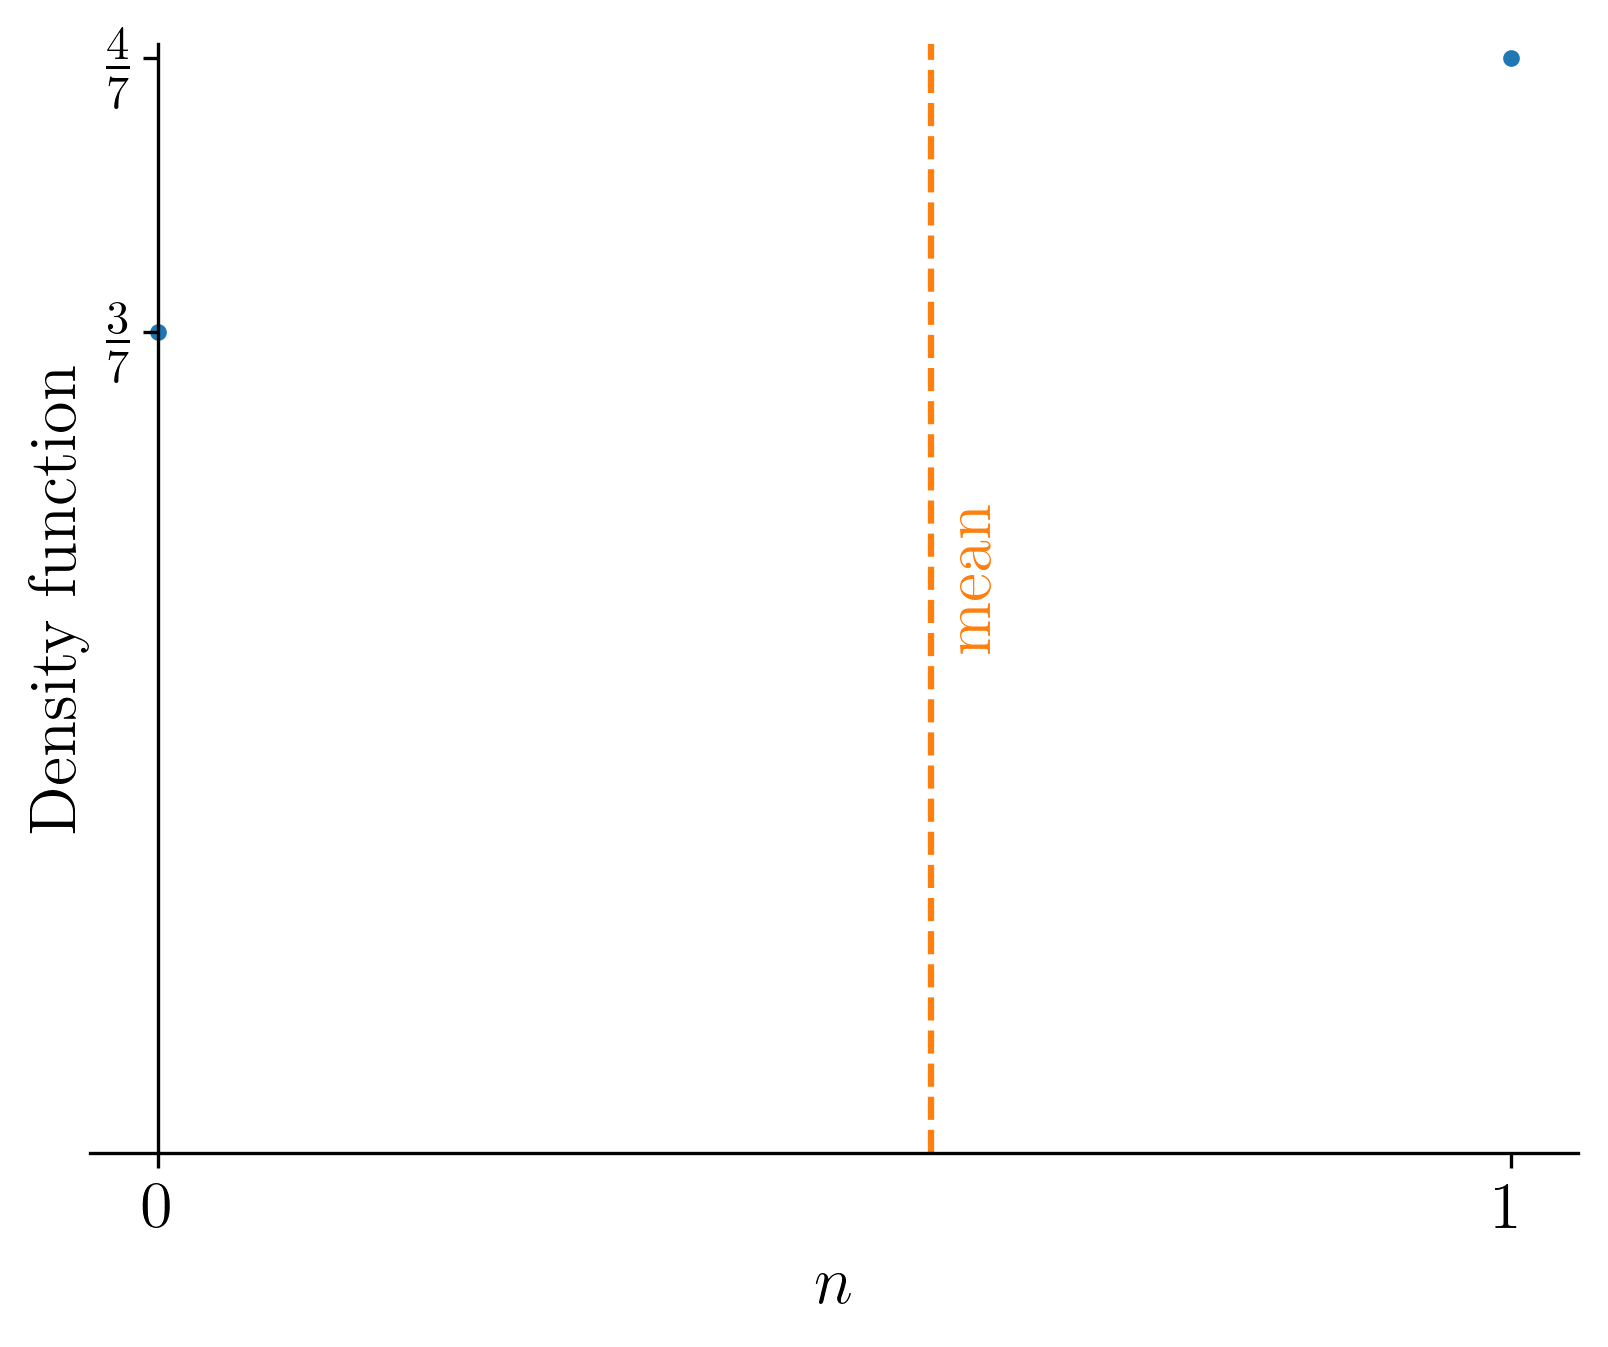
\includegraphics[width=\linewidth]{./Section/Momente/Erwartungswert Bernoulli.png}
\caption{\centering Dichte einer $\Ber(4/7)$-Verteilung}
\end{center}
\end{figure}
\end{minipage}
\begin{minipage}{0.5\linewidth}
\begin{figure}[H]
\begin{center}
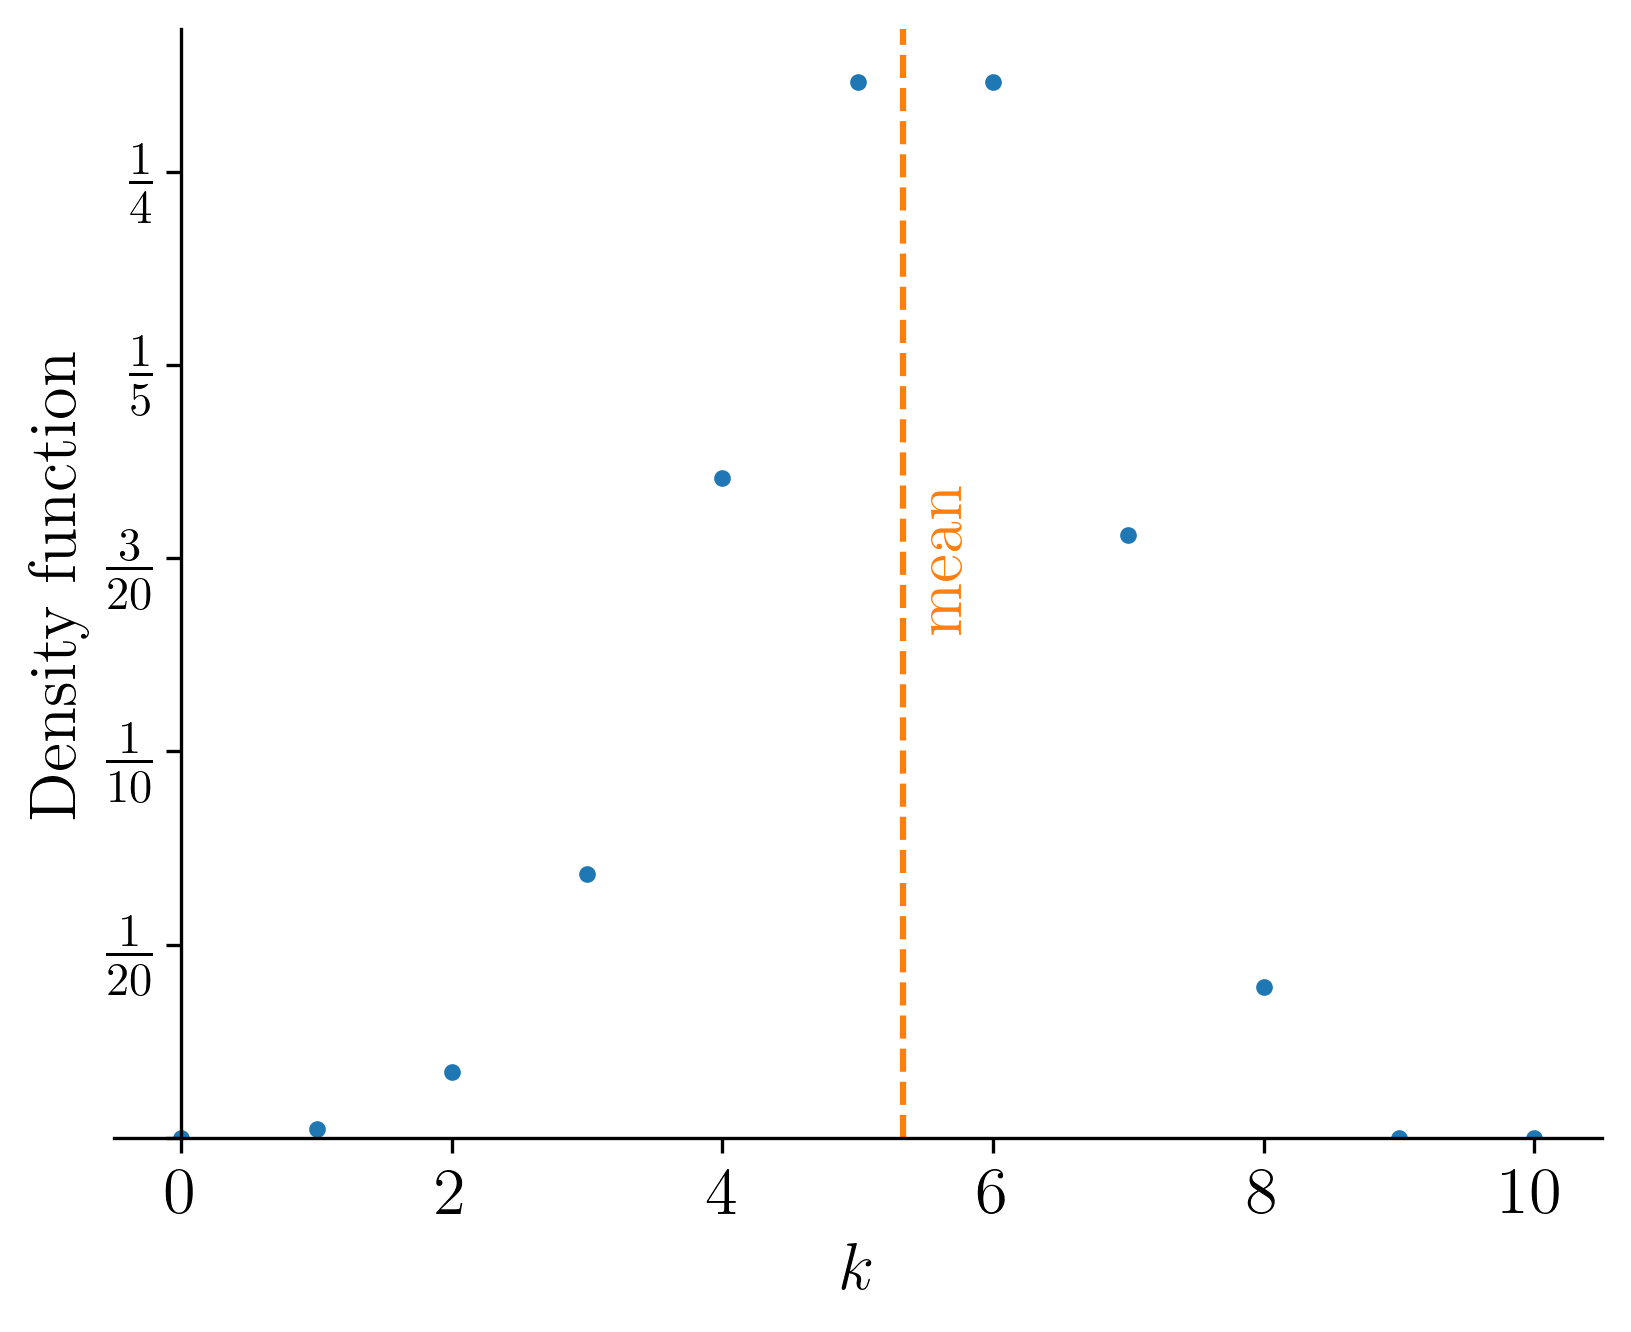
\includegraphics[width=\linewidth]{./Section/Momente/Erwartungswert Binomial.png}
\caption{\centering Dichte einer $\Bin(8, 2/3)$-Verteilung}
\end{center}
\end{figure}
\end{minipage}
\begin{minipage}{0.5\linewidth}
\begin{figure}[H]
\begin{center}
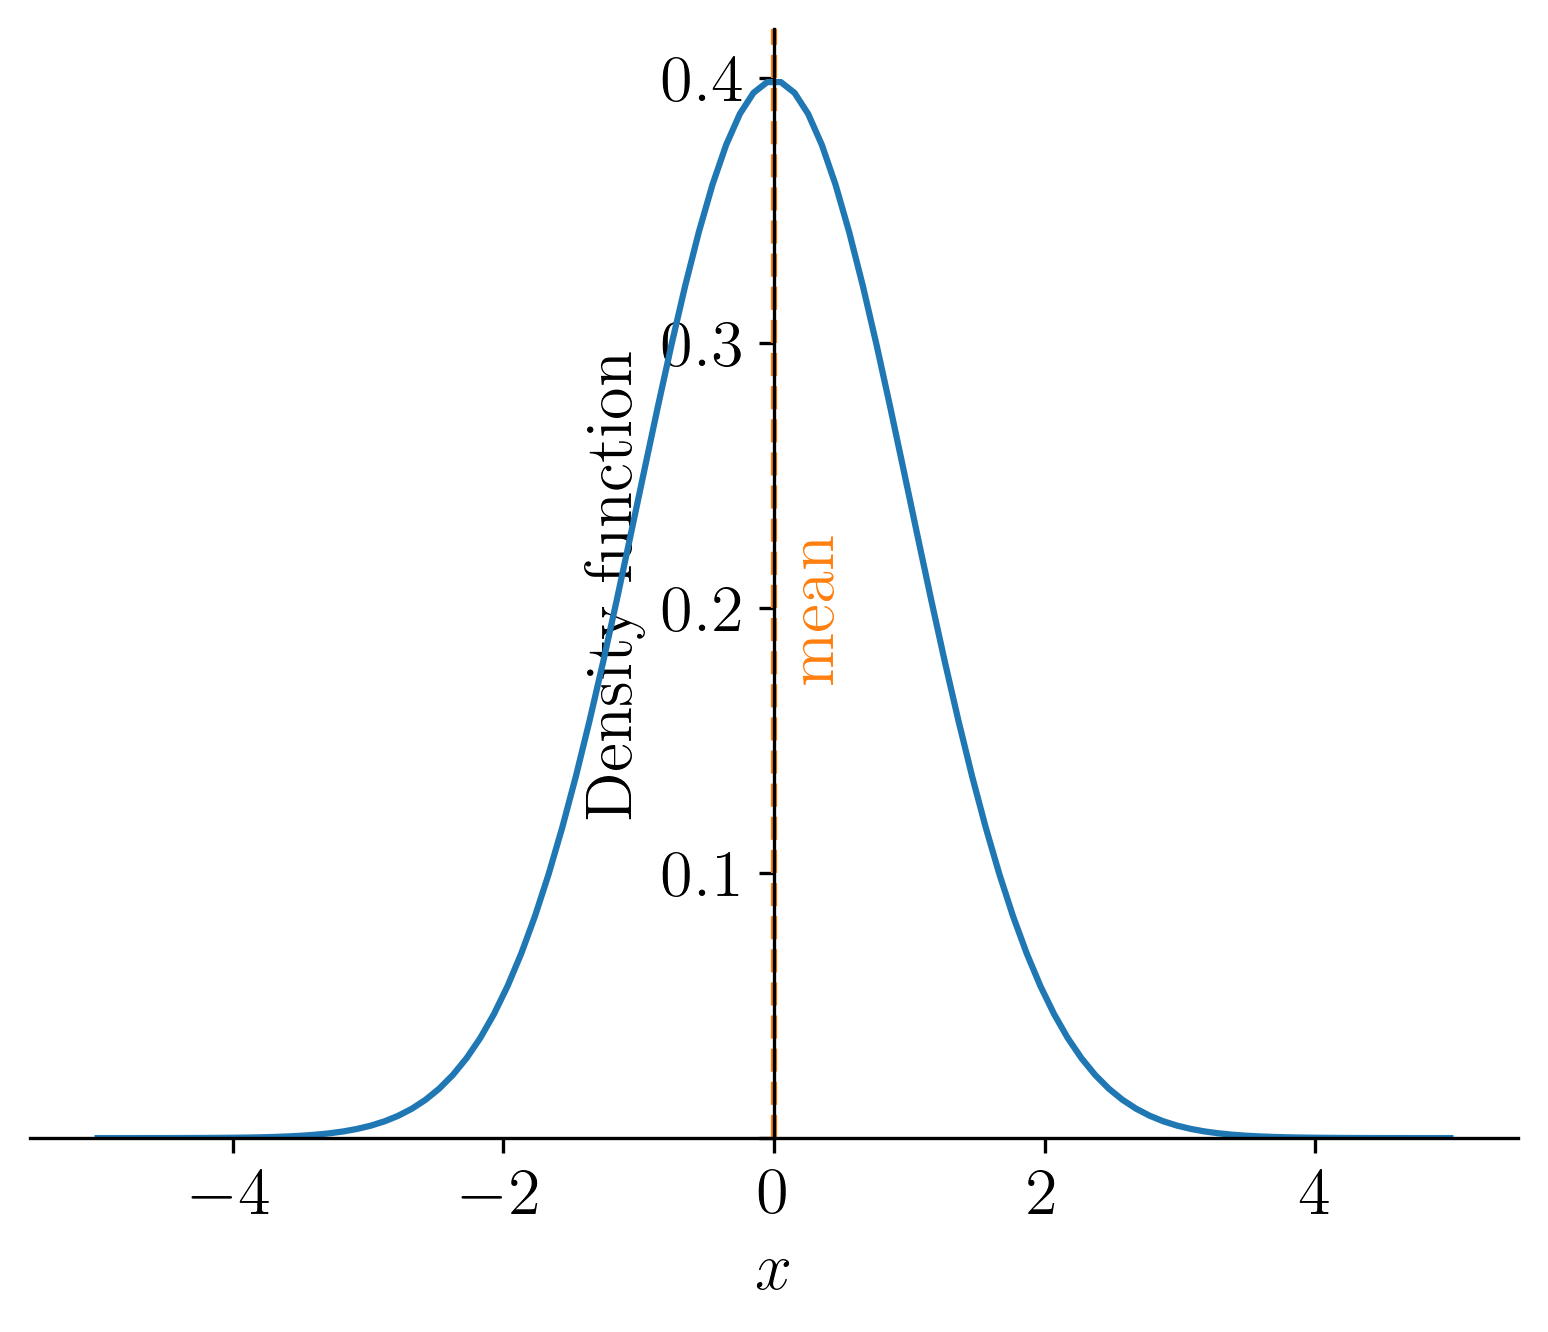
\includegraphics[width=\linewidth]{./Section/Momente/Erwartungswert Normal.png}
\caption{\centering Dichte einer $\Nor(0, 1)$-Verteilung}
\end{center}
\end{figure}
\end{minipage}
\begin{minipage}{0.5\linewidth}
\begin{figure}[H]
\begin{center}
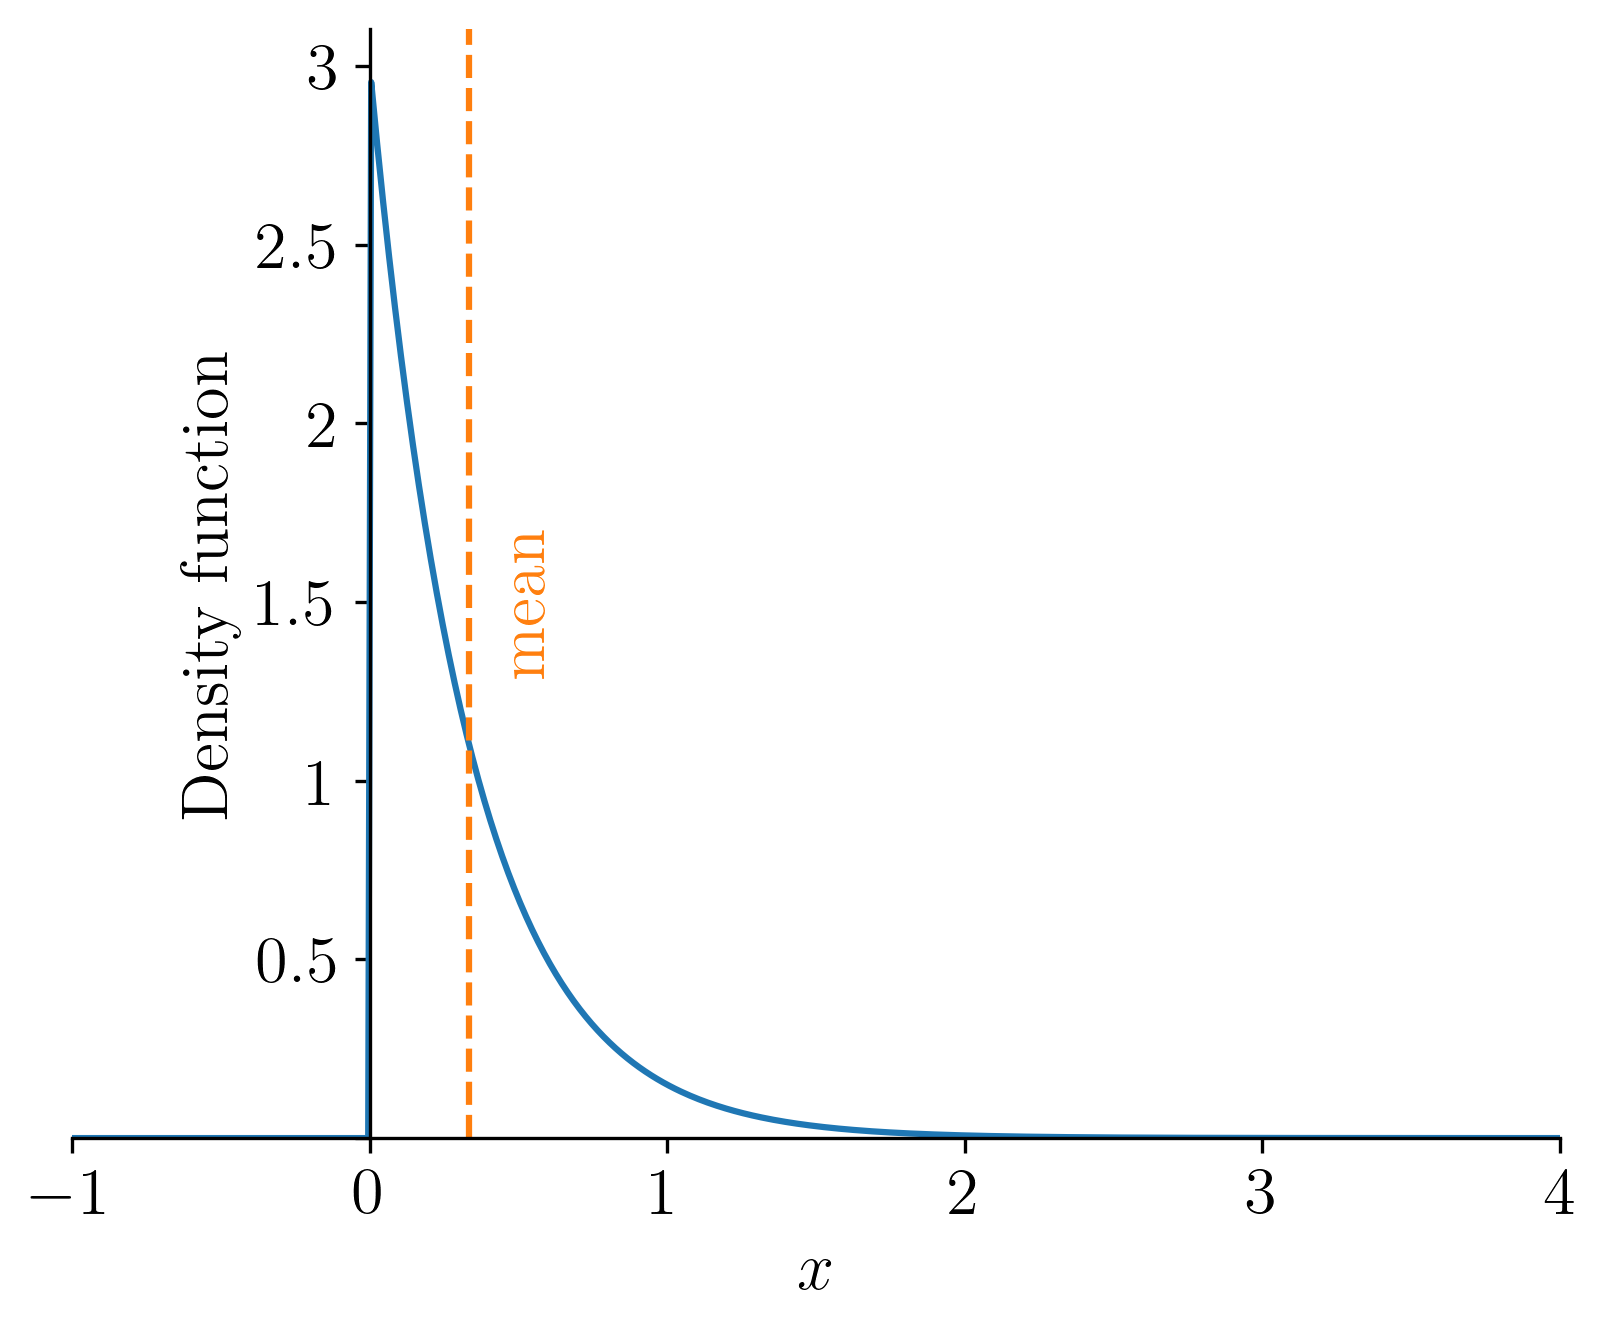
\includegraphics[width=\linewidth]{./Section/Momente/Erwartungswert Exponential.png}
\caption{\centering Dichte einer $\Exp(3)$-Verteilung}
\end{center}
\end{figure}
\end{minipage}

Wir sehen, dass der Erwartungswert tatsächlich die Verteilung teilt. Bei der finiten und diskreten Verteilung fällt auf, dass der Erwartungswert nicht unbedingt ein Wert sein muss, den die Zufallsvariable tatsächlich annimmt. Hierzu könnte man den Median \en{median} oder Modus \en{mode} berechnen.

\newpage 

Da die Dichtefunktionen von Normalverteilungen symmetrisch um den Erwartungswert sind, wollen wir diese noch gesondert betrachten.

\begin{figure}[H]
\centering
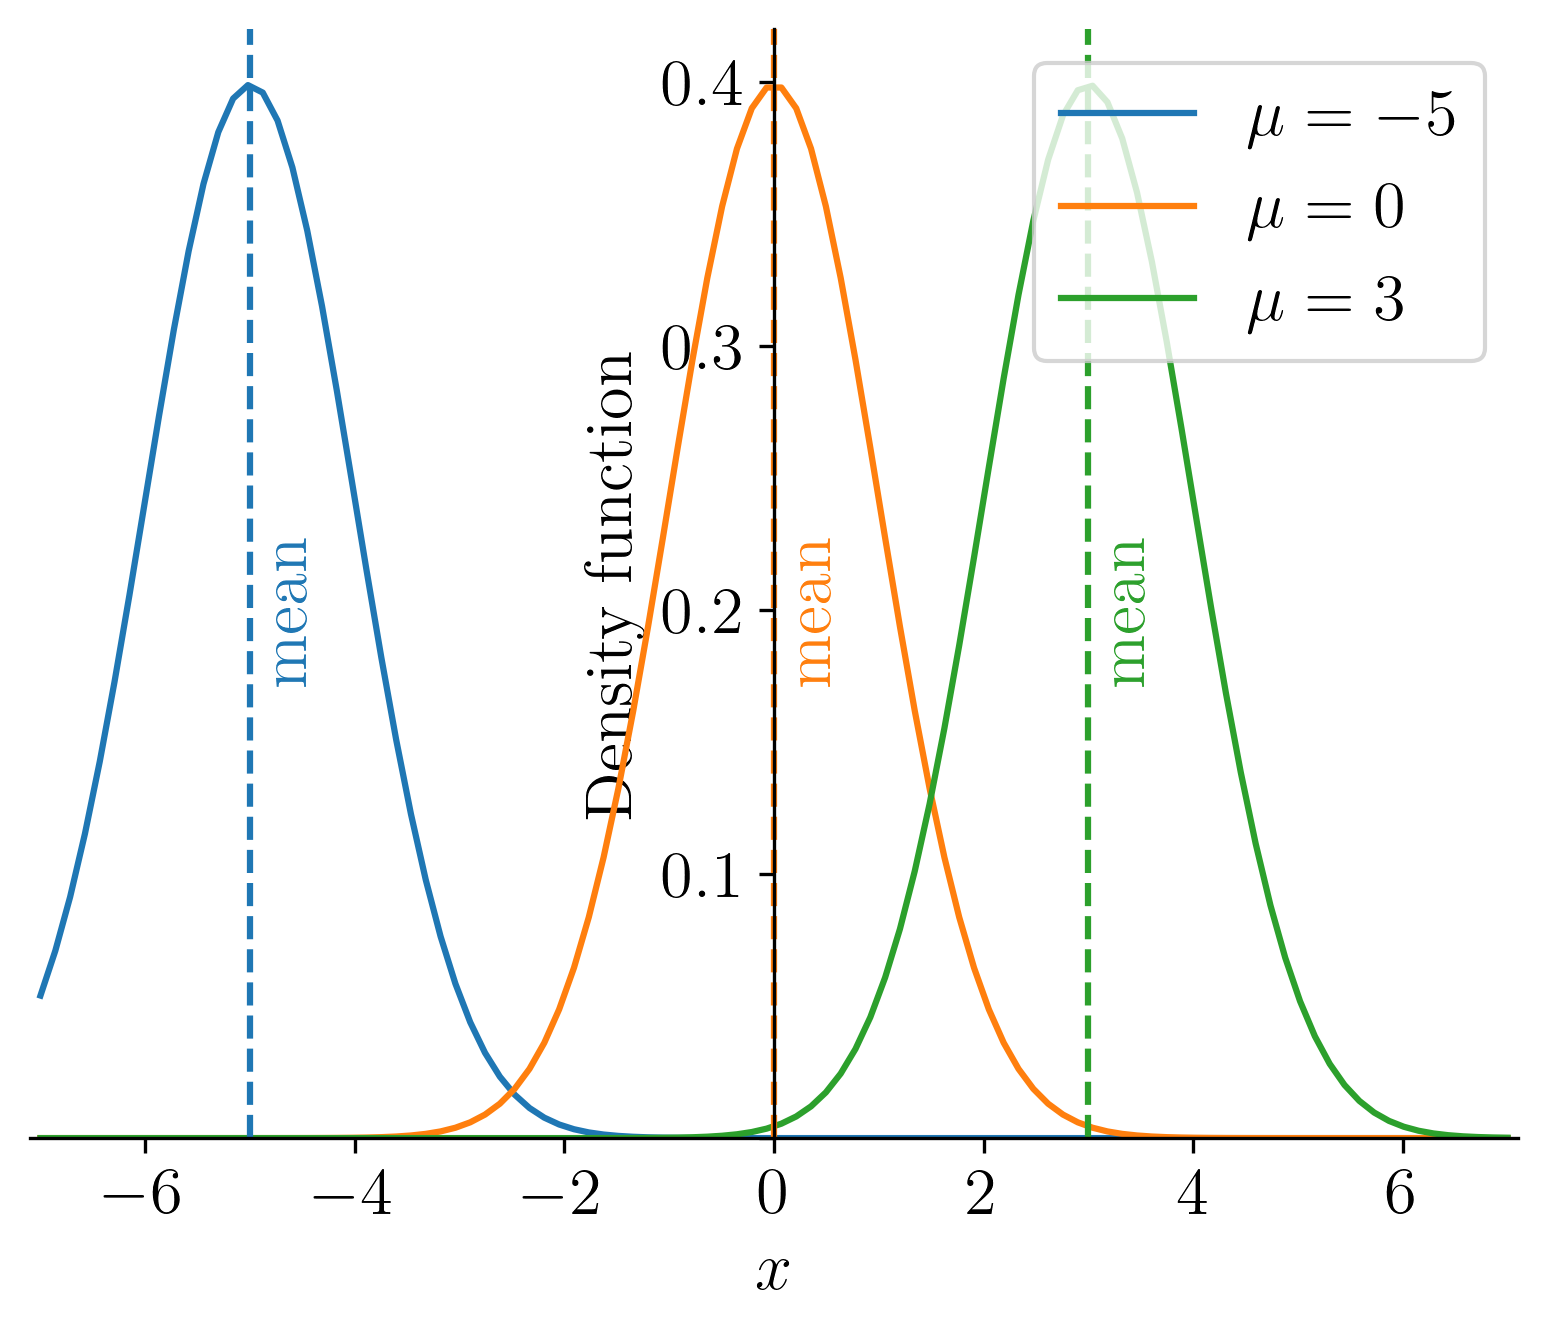
\includegraphics[width=0.5\linewidth]{./Section/Momente/Erwartungswert Normal Multi.png}
\caption{Dichte einer $\Nor(\mu, 1)$-Verteilung}
\end{figure}

Wir sehen also, dass Symmetriezentrum und Erwartungswert bei diesen Normalverteilungen zusammenfallen. Diese Aussage gilt sogar allgemein.
\end{Beispiel}

\vspace*{-\medskipamount}

\begin{Satz}{(Erwartungswert symmetrischer Verteilungen)}
Sei $(\Omega, \mathscr{A}, \mathbb{P})$ ein Wahrscheinlichkeitsraum und $X$ eine integrierbare Zufallsvariable, sodass die Dichte symmetrisch um $\mu$ ist. Dann gilt
\[\mathbb{E}(X) = \mu~.\]
\end{Satz}

\begin{Beweis}{}
Aufgrund der Symmetrie gilt
\[f(\mu + x) = f(\mu - x)\]
für alle $x \in \mathbb{R}$. Nach Definition gilt
\begin{align*}
\mathbb{E}(X) &= \int X \d \mathbb{P}\\
&= \int_\mathbb{R} x f(x) \d x~.
\intertext{Aufgrund der Integrierbarkeit können wir dieses Integral am Symmetriezentrum trennen und es gilt}
&= \int_{-\infty}^\mu x f(x) \d x + \int_\mu^\infty x f(x) \d x~.
\end{align*}
Wir werden nun diese beiden Integral getrennt voneinander betrachten. Betrachte zunächst
\begin{align*}
\int_{-\infty}^\mu x f(x) \d x &= \int_{-\infty}^\mu (\mu - (\mu - x)) f(x) \d x\\
&= \int_{-\infty}^\mu \mu f(x) - (\mu - x) f(x) \d x~.
\intertext{Dank der Linearität folgt}
&= \mu \int_{-\infty}^\mu f(x) \d x - \int_{-\infty}^\mu (\mu - x) f(x) \d x~.
\intertext{Das Integral im vorderen Summanden können wir auch mittels der Verteilungsfunktion $F_X$ ausdrücken}
&= \mu F_X(\mu) - \int_{-\infty}^\mu (\mu - x) f(x) \d x~.
\intertext{Auf eine ähnliche Weise betrachten wir das andere Integral}
\int_\mu^\infty x f(x) \d x &= \int_\mu^\infty (\mu + (x - \mu)) f(x) \d x\\
&= \int_\mu^\infty \mu f(x) + (x - \mu) f(x) \d x~.
\intertext{Mithilfe der Linearität folgt wieder}
&= \mu \int_\mu^\infty f(x) \d x + \int_\mu^\infty (x - \mu) f(x) \d x~.
\intertext{Im vorderen Integral finden wir die Gegenwahrscheinlichkeit zu vorigem Ereigniss. Wir können dies also umschreiben zu}
&= \mu (1 - F_X(\mu)) + \int_\mu^\infty (x - \mu) f(x) \d x~.
\end{align*}
Setzen wir diese Rechnung nun in die Berechnung des Erwartungswertes ein, so erhalten wir
\begin{align*}
\mathbb{E}(X) &= \mu F_X(\mu) - \int_{-\infty}^\mu (\mu - x) f(x) \d x + \mu (1 - F_X(\mu)) + \int_\mu^\infty (x - \mu) f(x) \d x\\
&= \mu - \int_{-\infty}^\mu (\mu - x) f(x) \d x + \int_\mu^\infty (x - \mu) f(x) \d x~.
\intertext{Aufgrund der Symmetrie der Dichtefunktion sind die beiden Integrale gleich und es gilt}
&= \mu~.
\end{align*}

Wir können diesen Satz auch auf eine deutlich elegantere und kürzere Art beweisen. Da $X$ symmetrisch bezüglich $\mu$ ist, haben $X - \mu$ und $\mu - X$ dieselbe Verteilung. Es gilt also
\[\mathbb{E}(X - \mu) = \mathbb{E}(\mu + X)~.\]
Damit gilt
\begin{align*}
0 &= \mathbb{E}(X - \mu) - \mathbb{E}(\mu - X)\\
&= \mathbb{E}(X - \mu - \mu + X)\\
&= \mathbb{E}(2 X - 2 \mu)\\
&= 2 \mathbb{E}(X) - 2 \mu\\
\intertext{und}
\mathbb{E}(X) &= \mu
\end{align*}
durch Umformen.
\end{Beweis}